%%%%%%%%%%%%%%%%%%%%%%%%%%%%%%%%%%%%%%%%%%%%%%%%%%%%%%%%%%%%
%%  This Beamer template was created by Cameron Bracken.
%%  Anyone can freely use or modify it for any purpose
%%  without attribution.
%%
%%  http://cameron.bracken.bz/beamer-template
%%
%%  Template Last Modified: January 9, 2009
%%

\documentclass[xcolor=x11names,compress]{beamer}

%% General document %%%%%%%%%%%%%%%%%%%%%%%%%%%%%%%%%%
\usepackage{graphicx}
\usepackage{tikz}
\usepackage[utf8]{inputenc}
\usepackage[labelformat=empty]{caption}
% For subfigure
\usepackage{subcaption}
\usetikzlibrary{decorations.fractals}
%%%%%%%%%%%%%%%%%%%%%%%%%%%%%%%%%%%%%%%%%%%%%%%%%%%%%%


%% Beamer Layout %%%%%%%%%%%%%%%%%%%%%%%%%%%%%%%%%%
\useoutertheme[subsection=false,shadow]{miniframes}
\useinnertheme{default}
\usefonttheme{serif}
\usepackage{palatino}

\usepackage{tikz}  

\setbeamerfont{title like}{shape=\scshape}
\setbeamerfont{frametitle}{shape=\scshape}

\definecolor{FEUPCor}{rgb}{0.54, 0.17, 0.09}
\setbeamercolor*{lower separation line head}{bg=FEUPCor} 
\setbeamercolor*{normal text}{fg=black,bg=white} 
\setbeamercolor*{alerted text}{fg=red} 
\setbeamercolor*{example text}{fg=black} 
\setbeamercolor*{structure}{fg=black} 
 
\setbeamercolor*{palette tertiary}{fg=black,bg=black!10} 
\setbeamercolor*{palette quaternary}{fg=black,bg=black!10} 

\addtobeamertemplate{navigation symbols}{}{%
    \usebeamerfont{footline}%
    \usebeamercolor[fg]{footline}%
    \hspace{1em}%
    \insertframenumber/\inserttotalframenumber
}
\setbeamercolor{footline}{fg=black}
\setbeamerfont{footline}{series=\bfseries}

%\setbeamertemplate{note page}[plain]

\renewcommand{\(}{\begin{columns}}
\renewcommand{\)}{\end{columns}}
\newcommand{\<}[1]{\begin{column}{#1}}
\renewcommand{\>}{\end{column}}
\renewcommand{\footnotesize}{\scriptsize}
%%%%%%%%%%%%%%%%%%%%%%%%%%%%%%%%%%%%%%%%%%%%%%%%%%

\title{\texorpdfstring{From Simulation to Development in MAS:\\
		A JADE-based Approach}{}}
\author{\texorpdfstring{João Pedro Camacho Lopes\\
		Orientador: Henrique Lopes Cardoso}{}}

\begin{document}


%%%%%%%%%%%%%%%%%%%%%%%%%%%%%%%%%%%%%%%%%%%%%%%%%%%%%%
%%%%%%%%%%%%%%%%%%%%%%%%%%%%%%%%%%%%%%%%%%%%%%%%%%%%%%
\begin{frame}

\includegraphics[height=0.7cm]{figures/uporto-feup.pdf}\\

%\subtitle{SUBTITLE}
\vspace{1cm}

\date{14 de Julho 2014}
\titlepage
\end{frame}

\section{Introdução}
%!TEX root = ../thesis.tex
\chapter{Introduction}
\label{chap:introduction}
%<In this paragraph present the context of the thesis, introducing the subject of MAS, MABS and some of their uses. Refer that standards exist and why. Introduce the next sections too.>
Multi-Agent Systems (MAS) are composed of autonomous computational elements capable of interacting with each other, called agents. The development of this class of systems comprises an interesting software paradigm but in terms of computer science history, MAS are a recent subject, having gained significant traction only after the mid 1990's \cite{wooldridge2008introduction}. With multiple applications such as problem solving, simulation, trading, negotiation, computer games and logistics using an efficient and modular development approach, MAS enjoyed a rapid growth in popularity and are in widespread use nowadays \cite{ferber1999multi}.

Presently, tools and frameworks for the development of all sorts of MAS are as diverse as uses exist for them. This thesis describes a concrete problem of integrating frameworks from different domains.

\section{Problem}
%The following problems will be explained:

% - There is no universal standard. Most systems don't use any standards
Although their use is certainly widespread, there is no universal general purpose standard for MAS development, since each system has different needs. Many times, such systems are created from scratch, meaning that the developers must define all features of the system - such as its agents, their behaviour, communication and organization, using conventional programming languages and tools. However, several frameworks exist that offer some level of abstraction from the code, allowing for a more conceptual approach to
MAS development \cite{gormer2011jrep}. 

% - Full featured MAS development frameworks are often not the most appropriate to develop simulations for their complex architecture
Most uses of MAS, for instance in negotiation, games or logistics, demand a small number of agents, typically with larger resource demands but without any need for global control of execution, i.e. it is perfectly reasonable for these types of systems to be based on events and for its agents to work asynchronously. In contrast, Multi-Agent-Based Simulations (MABS) are usually implemented using a large number of lightweight agents with a small resource footprint. MAS development frameworks generally provide the programmer with a range of features such as execution control, communication protocols or agent awareness capabilities. In spite of that, most frameworks that focus on MAS development lack synchronization mechanisms and lightweight agent infrastructure required by MABS. One of the main goals of simulations is to be able to visualize real-time, as well as historical data that allow to study emergent and evolutionary phenomena. \cite{mengistu2008scalability}

% - Porting code from one framework to the other is typically not a feasible solution 
When an application has been developed using a MAS development framework and a need later arises for the creation of simulations, porting the source code to an appropriate MABS development framework is a labour-intensive task since not only the syntax and API of the new framework is significantly different, but conceptually speaking, the adaptation may require significant changes to the application.


\section{Motivation}
% It is useful that MAS be tested in a controlled simulation environment using proper simulation tools that may not be available in their destination platform;
Interest exists in the simulation of MAS. At any point of the development of the system, it may be valuable to test MAS in a local and controlled simulation environment and to take advantage of some features present in MABS frameworks that are not available in the destination platform of the system.The rationale for the creation of simulated agent systems is usually concerned with simulation performance. Simulations typically have a higher performance than complex MAS frameworks. For many popular MAS frameworks, there is an opportunity to gain performance when executing tests and simulations. 

% JADE and Repast are popular tools in widespread use and are well documented and supported by their communities so it is easier to build on top of them;
% "It is feasible to bridge the gap between MAS simulation and development by embedding FIPA-standards and JADE features in a simulation framework."
% "The development of a robust MAS can be partially automated from a previously tested simulation."
As some works suggest \cite{gormer2011jrep,garcia2011misia,warden2010towards}, it is feasible to bridge the gap between MAS simulation and development. For instance, JADE and Repast are popular tools in widespread use and are well documented and supported by their communities so it is easier to build on top of them. It it possible to establish this bridge by embedding FIPA-standards and JADE features in Repast.

\section{Goals}
The main goal of this thesis was to develop a code conversion tool. In order to bring MAS development and simulation together, this tool would allow to convert the code written for a development tool into code for a simulation tool. 

JADE and Repast were chosen over other platforms mainly for their popularity and widespread use - not dismissing their quality, of course. As an example of an alternative framework, Cougaar (Cognitive Agent Architecture)\cite{helsinger2004cougaar} solves the problem explain above by proposing a fully featured agent architecture, while maintaining high performance and scalability required for simulation. It doesn't, however, implement any interaction standards; messages are exchanged by means of serialized Java objects. Therefore, another goal was to develop an API that replicates the essential JADE features, while abdicating of JADE's networking infrastructure and more complex internal features in favour of gaining in simulation performance. This includes enabling interaction standards in simulation frameworks. While Repast is the featured framework for simulation development, it was part of this goal to develop an API that was sufficiently generic to allow for future enhancements and support for new platforms.

Programmers that wish to use the code conversion tool should not be forced to introduce significant changes to the original code in order to be able to use the tool. The goal was that the tool should be capable of converting the code \emph{as-is} and generate working models. The generated code must also preserve the functionality of the original code - meaning that the re-conversion must generate code that is equivalent to the original one.

% To enable interaction standards in simulation frameworks;
% To develop an API that replicates the essential JADE features, while abdicating of JADE's networking   infrastructure and more complex internal features in order to gain in simulation performance;
% To develop an automatic code conversion tool (CCT) that uses this API to transform Repast-based simulations into JADE MAS;
% To add the possibility to convert some JADE MAS into simulations, based on the API and using the code conversion tool;
% To validate generated code by confirming that the execution of the simulation and the generated MAS produce identical behaviour;
% To make the API generic enough, allowing for future extension to support multiple simulation tools

\section{Contents}

This thesis documents the development of a tool that converts a MABS created in Repast into MAS that uses JADE. Conversely, it should allow the conversion of a JADE MAS into a Repast MABS as well. This tool is useful in the context of development of a MAS whose development started as a MABS or when the need to create a simulation arises during development. JADE and Repast were chosen for this thesis not only for their quality but also for their widespread use, available source code and documentation.

Chapter \ref{chap:background} starts by surveying tools whose goal is to produce MABS. Three frameworks were selected for a more detailed study because their approach is the most relevant to the goals of this thesis. They propose solutions based on enhancing JADE to enable simulations capabilities in it. The rest of the chapter is dedicated to comparing JADE and Repast's features and to include an introduction to some concepts regarding FIPA specifications.

Chapter \ref{chap:solution} provides a conceptual definition of the developed tools, including an overview of their features and usage scenarios. This chapter also describes how FIPA Specifications are present in the API. To better understand how the code conversion tool, some background study is presented before describing the features of tool.

Chapter \ref{chap:architecture} gives a detailed description of the software architecture, including a description of how agents execute internally, in the API. This chapter is concluded with a discussion on the perspectives for extending the tools, teasing for the discussion of future work in Chapter \ref{chap:futurework}.

Chapter \ref{chap:validation} presents scenarios used to validate the system. They were subjected to code conversion to verify that the correct execution of the code had been preserved. Their performance was also subject to analysis.

This thesis is concluded with a description of suggested future work and some final notes and conclusions.

\section{Estado da Arte}
%!TEX root = ../thesis.tex
\chapter{Background}
\label{chap:background}

Studying ways to bridge the gap between the fields of MAS and MABS has been the subject of several works and resulted in the development of different tools, each with its own purpose. Some works were in search of increased performance for MABS; others tried to cater specific needs such as providing an appropriate learning environment. This chapter describes some works that are relevant to this thesis and makes a comparison between some of them.

\section{Related Work}
% Study of similar frameworks for agent based simulation
Several frameworks exist that offer support to the development of MAS or MABS. Some are domain specific, meaning that their purpose was well defined in their conception. MASeRaTi\cite{ahlbrecht2014scalable}, MATSim\cite{balmer2008agent} and SUMO\cite{SUMO2012} are some examples of MABS frameworks for traffic and transports simulation. 

Other works like Repast\cite{collier2003repast}, NetLogo\cite{tisue2004netlogo}, GALATEA\cite{davila2000galatea} and Plasma \cite{warden2010towards} are considered general-purpose. This list comprises only tools that are free and open source and is not meant to be exhaustive. 

Some works propose approaches that are very similar to the solution proposed in this thesis, namely the bridging of the domains of MAS and Simulation. MISIA, JRep and Plasma were built on top of JADE to create a simulation environment based on it. These three works were studied with more detailed due to these similarities.

\subsection{MISIA}
MISIA is a middleware whose goal is to enhance the simulation of intelligent agents and to allow the visualization and analysis of agent's behaviour. It was developed by the Bioinformatic, Intelligent Systems and Educational Technology Research Group (BISITE) from Universidad de Salamanca\footnote{http://bisite.usal.es/}. It is no longer an active project; as a research experiment, work on this middleware evolved into other more specific tools.

MISIA's approach, as suggested by Figure \ref{fig:misia}, is to use a middle layer that acts as the bridge between two other layers that interact with JADE and Repast. By extending the agents in Repast and JADE, communicating through a coordinator and synchronizing their state, these agents work as a single one.

\begin{figure}[h]
	\centering
	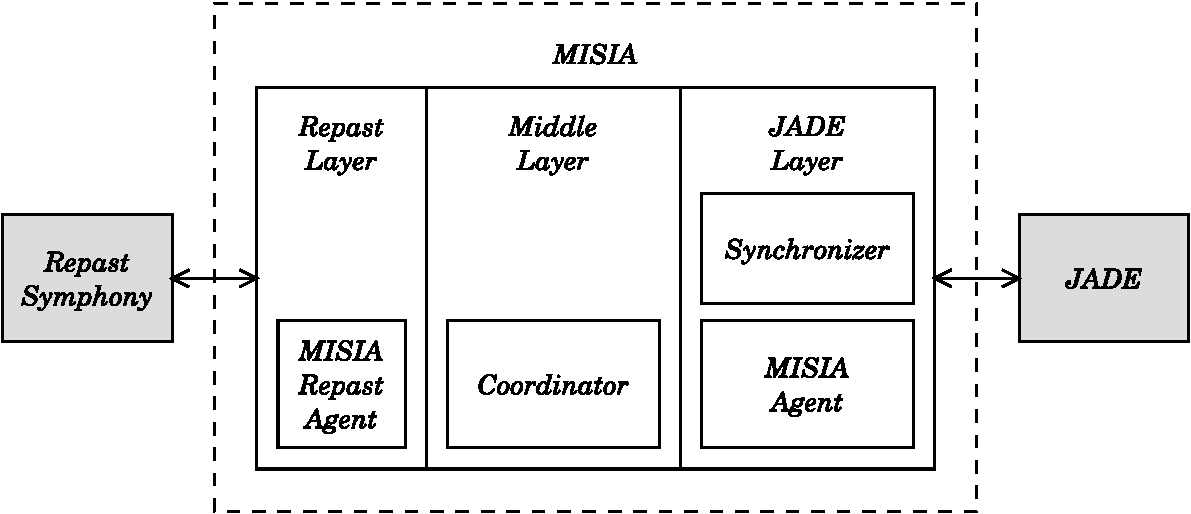
\includegraphics[width=0.75\linewidth]{figures/MISIA.pdf}
	\caption[MISIA's architecture]{High-level representation of MISIA's architecture (adapted from \cite{garcia2011misia})}
	\label{fig:misia}
\end{figure}

One of the challenges identified by the authors when re-implementing the FIPA interaction protocols was synchronizing them with the Repast tick-based simulation model. Given JADE's event-driven architecture, MISIA proposes the use of a coordinator agent that informs the JADE-Agent when a tick has passed. It also proposes its own implementation of the interaction protocols supported by JADE, making them tick-friendly.

\subsection{JRep}
JRep is another platform for integrating JADE and Repast Symphony in the same framework, by means of a middleware. To demonstrate its use, the authors present an example of a smart airport and how it can be simulated using JREP.

JRep's approach is not as complex as MISIA's.
By having the Repast Simphony agent encapsulate a JADE agent representation, synchronization is immediate and is assured without requiring an external coordinator.
The two agent representations take care of synchronizing any state changes.
Figure \ref{fig:jrep} represents the basic structure of JRep.

\begin{figure}[h]
	\centering
	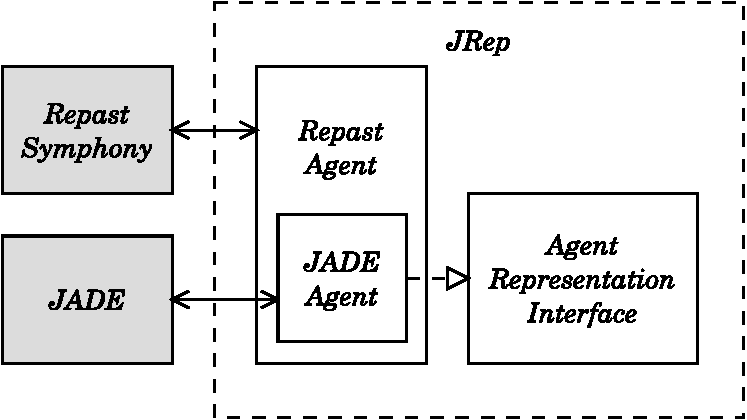
\includegraphics[width=0.5\linewidth]{figures/jrep.pdf}
	\caption[JRep's architecture]{High-level representation of JRep's architecture (adapted from \cite{gormer2011jrep})}
	\label{fig:jrep}
\end{figure}

Each agent takes care of interfacing their respective frameworks. The interaction between agents in JRep is performed using FIPA ACL and the protocol implementations are those provided by the JADE platform. Similarly to MISIA, an Agent Representation Interface is used to introduce the concept of schedule in the JADE agent.

\subsection{PlaSMA}
Unlike the two previous frameworks, the PlaSMA system is based solely on the JADE platform. The distributed simulation is synchronized by entities called ``Controllers'' who communicate with the ``Top Controller'', keeping the pace of the simulation and handling agent lifecycle management as well. Figure \ref{fig:plasma} illustrates this architecture. PlaSMA, unlike MISIA and JRep, is still an active project.

\begin{figure}[h]
	\centering
	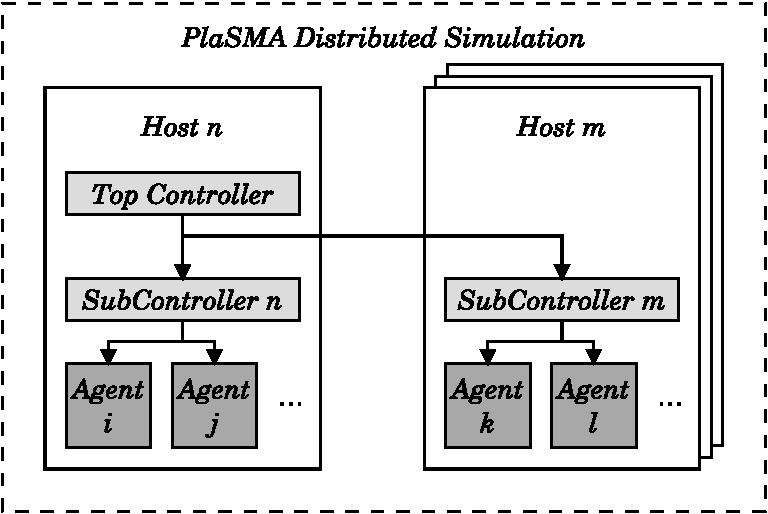
\includegraphics[width=0.5\linewidth]{figures/PlaSMA.pdf}
	\caption[PlaSMA's architecture]{High-level representation of PlaSMA's architecture (adapted from \cite{warden2010towards})}
	\label{fig:plasma}
\end{figure}

JADE is a very rich platform but, for many simulation scenarios, the overhead introduced by it has a significant impact on simulation performance \cite{mengistu2008scalability}.

Even though both MISIA and JRep attempt to integrate the features from both JADE and Repast, as far as Repast simulations are concerned JADE's multi-threaded infrastructure affects their performance very significantly. The main advantage of our approach is, therefore, the possibility of using Repast with JADE features, namely FIPA specifications including interaction protocols, without the need to interface with JADE. 

\section{JADE and Repast}
\label{sec:jade-repast}

To achieve the goals of this thesis, two frameworks were chosen: JADE and Repast. Both are very popular and in widespread use and have been the foundation of the creation of other tools. They are also free and open source and extensively documented.

JADE is a framework for development of FIPA-compliant fully featured MAS. It aims at simplifying the creation of distributed agent applications by seamlessly hiding all complexity regarding its distributed architecture, including the tasks of agent discovery and the handling of messages.

Repast is a toolkit that provides an environment for the creation of MABS using POJO\footnote{Plain Old Java Objects}. It makes it fairly simple to collect agent data and generate displays for it, including charts, grids and others.

\begin{table}[h]
	\caption{Summary of JADE and Repast features.}
	\label{tab:jadevsrep}
	\begin{center}
		\begin{tabular}{l|cc}
		\hline

		\hline
		\textbf{} & \textbf{JADE} & \textbf{Repast} \\ %& \textbf{Cougaar} \\
		\hline
			Communication & FIPA ACL &  Method calls  \\ %& Serialized Object \\
						  &			 &  Shared resources \\
		\hline
			Distribution & Yes & No \\ %& Yes \\
		\hline
			Simulation Tools & No & Yes \\ %& Yes \\
		\hline
			Scalability & Limited & High \\ %& High \\
		\hline
			Ontologies & Yes & No \\ %& Yes\\
		\hline
			Open Source & Yes & Yes \\ %& Yes\\
		\hline
			Agent Execution & Behaviour-based & Schedule-based  \\ %&  \\
							& Multi-threaded & Single-threaded \\ %&  \\
							& Event-driven   & Tick-driven 	   \\ %&  \\
							& Assync		 & Sync 		   \\ %&  \\
		\hline
		\end{tabular}
	\end{center}
\end{table}

In JADE, as table \ref{tab:jadevsrep} illustrates, agents execute in separate threads and while this architecture facilitates the platform's distribution, JADE's agent are heavy in terms of resources. Experiments with JADE show that the platform's scalability is limited in number of agents and that the global system performance drops quickly for large number of agents \cite{mengistu2008scalability} \cite{garcia2011misia}. This further strengthens the idea that using JADE or a JADE-Repast hybrid, as describe in the related work, is not the best course of action is performance is an important issue.

In Repast, agent execution is scheduled manually. An agent class can contain annotations that indicate which methods should be called and when (for instance every tick or every 100 ticks). This approach is very flexible, allowing to schedule any method but more complex structures are non-existent in Repast.

In contrast, JADE agent actions can be executed in their setup and takedown, but most are encapsulated in objects called Behaviours. JADE has many different kinds of behaviours that function in different ways, such as running one single task once or running them cyclically. Other behaviours implement FIPA interaction protocols, which agents can use to interact with other agents.

Agents, as well as their behaviours, go through different states, as Figure \ref{fig:jade_fluxogram} suggests. As each agent in JADE runs in a thread, each one is dedicated solely to the agent's behaviours. These behaviours are executed consecutively until the agents is taken down and each behaviour stops being scheduled when it is ``done'' -- indicated by the return value of the method \texttt{done()}.

\begin{figure}[h]
	\centering
	\includegraphics[width=0.7\linewidth]{figures/jade_fluxogram.pdf}
	\caption[JADE Behaviour execution states]{JADE Behaviour execution states and events (adapted from \cite{bellifemine2007developing})}
	\label{fig:jade_fluxogram}
\end{figure}

%!TEX root = ../thesis.tex
\section{FIPA Specifications in JADE} % (fold)
\label{sec:fipa}

% Intro to FIPA in JADE/API
\apiname{} closely follows JADE's architecture regarding the use of protocols and services specified by FIPA. 
%The architecture of the API described in this paper includes multiple concepts proposed by FIPA: the \gls{DF}, the \gls{MTS}, the \gls{AMS}, the \gls{ACL} Message and the Interaction Protocols. The following is a brief description of these concepts and of how JADE uses and implements them.

%\begin{figure}
%	\centering
%	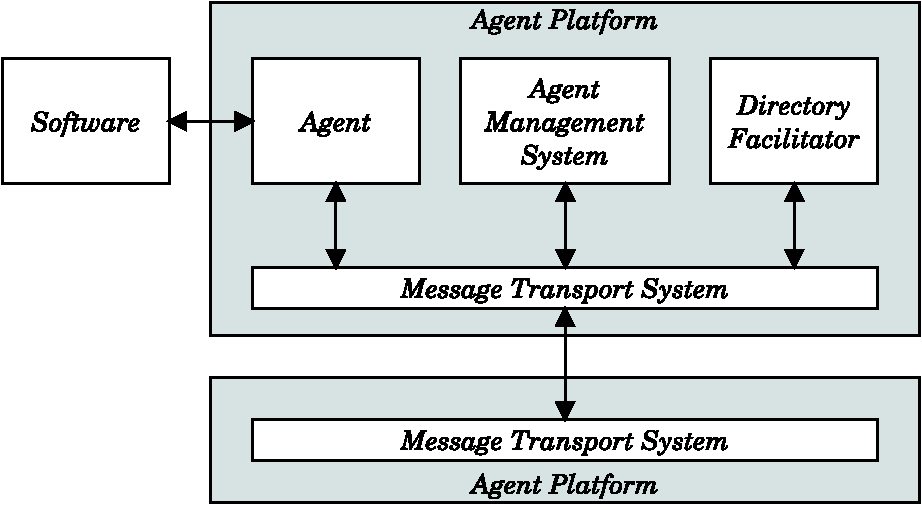
\includegraphics[width=2.5in]{figures/pdf/AMSdiagram.pdf}
%	\caption{
%		Agent Management Reference Model, as specified by FIPA and implemented by JADE. \apiname{} only supports a single Agent Platform.
%	}
%	\label{fig:AMSdiagram}
%\end{figure}

% DF 
The Directory Service (DF) is a component that provides a yellow page service and is part of the FIPA Agent Management Specification. It allows one agent to perform searches about agents rendering specific services. Only agents that are registered in the DF will be indexed and agents can register and deregister themselves at any time.

% DF Agent Description
When searching the DF, agents can use templates that filter the search results. A DF Agent Description represents this template and contains the fields listed in Table \ref{tab:dfAgentDescription}.sim


% MTS
The MTS is a service for transportation of ACL messages between agents. It is responsible for resolving agent addresses, in order to be able to deliver those messages. The MTS may request information from the AMS to perform this address resolution.

% AMS
The AMS is a mandatory component in FIPA-compliant agent platforms. Its purpose is to manage the agent platform, namely the creating and deletion of agents.

% ACL Message
The ACL Message is the envelope that contains the details for communication. The Agent Comunication Language (ACL) stipulates what fields a message should contain. Table \ref{tab:fipaACLMessage} was adapted from the FIPA ACL Message structure specification and contains the list of fields in a message. Not all of them are mandatory. FIPA specifies the \texttt{performative} as the only mandatory field, although the \texttt{sender}, \texttt{receiver} and \texttt{content} are expected to be present.

\begin{table}
	\normalsize
	\caption{FIPA ACL Message Parameters}
	\label{tab:fipaACLMessage}
	\begin{center}
		\fboxsep1pt
		\begin{tabular}{c|c}
		\hline
		\textbf{Parameter} & \textbf{Category of Parameters} \\
		\hline
		\colorbox{Apricot}{\texttt{performative}} & Type of communicative acts \\
		\hline
		\colorbox{Apricot}{\texttt{sender}} & \multirow{3}{*}{Participant in communication} \\
		\cline{1-1}
		\colorbox{Apricot}{\texttt{receiver}} \\
		\cline{1-1}
		\texttt{reply-to}  \\
		\hline
		\colorbox{Apricot}{\texttt{content}} & Content of message \\
		\hline
		\texttt{language} & \multirow{3}{*}{Description of Content} \\
		\cline{1-1}
		\texttt{encoding} \\
		\cline{1-1}
		\colorbox{Apricot}{\texttt{ontology}} \\
		\hline
		\colorbox{Apricot}{\texttt{protocol}} & \multirow{5}{*}{Control of conversation} \\
		\cline{1-1}
		\colorbox{Apricot}{\texttt{conversation-id}} \\
		\cline{1-1}
		\texttt{reply-with} \\
		\cline{1-1}
		\texttt{in-reply-to} \\
		\cline{1-1}
		\colorbox{Apricot}{\texttt{reply-by}} \\
		\hline
		\end{tabular}
	\end{center}
\end{table} 

% Protocols In FIPA
FIPA Interaction Protocols typify communication interactions among agents by specifying two roles: initiator (the agent starting the interaction) and responder (a participant in the interaction). Each protocol defines precisely which messages are sent by each role ad in which sequence.

% Behaviors in JADE
In JADE, every agent activity is programmed through the notion o behaviours. For interaction protocols, typically behaviour-pairs are used for each side of the interaction, and JADE's API supports the most important protocols with built-in initiator and responder behaviours.
% Implementing these protocols.
In order to create an application using these protocols, programmers only need to extend these behaviours and implement the message handlers.
All the complexity regarding the interaction and networking infrastructure is hidden and taken care of by JADE, allowing the programmer to focus on the implementation of agent behaviour.

\subsection{FIPA Interaction Protocols}

To provide a more solid background to the protocols mentioned in this thesis, it's relevant to perform a deeper analysys of them. The two protocols currently supported in the API, as will be explained further ahead in Chapter \ref{chap:solution}, are the FIPA Request, FIPA Query and the FIPA Contract Net. JADE supports a few other protocols, namely FIPA Propose, Iterated FIPA Request and Query and FIPA Subscribe.

\begin{table}
	\normalsize
	\caption{Interaction protocols supported in JADE}
	\label{tab:fipa_protos}
	\begin{center}
		\fboxsep1pt
		\begin{tabular}{c|c|c}
		\hline
		\textbf{Protocol(s)} & \textbf{Initiator class} & \textbf{Initiator class} \\
		\hline
		FIPA request 	& \multirow{2}{*}{AchieveREInitiator} & \multirow{2}{*}{AchieveREResponder}\\
		FIPA Query 		& \\
		\hline
		\multirow{2}{*}{FIPA Contract Net} & \multirow{2}{*}{ContractNetInitiator} & ContractNetResponder \\
		 &  & SSContractNetResponder \\
		\hline
		\end{tabular}
	\end{center}
\end{table}


In JADE, the AchieveRE protocol encompases the multiple ``request-like'' behaviours such as FIPA-Request. It is a simple protocol with three moments of interaction, as Figure \ref{fig:FIPA_request_proto} shows: a request, a response of acceptance or refusal and a facultative result notification. JADE allows the use of other interaction protocols with the AchieveRE: FIPA-query, FIPA-Request-When, FIPA-recruiting and FIPA-brokering. Interaction using this protocol can be 1:1 or 1:N.

The Contract Net protocol starts with a Call for Proposals (CFP) sent to one or more agents, which can reply with a proposal or with a refusal to propose. The initiator can then accept or reject the proposals. As in FIPA-Request, the final result notification is facultative. The ContractNetResponder class from JADE resets itself after terminating the protocol and stays waiting for new CFPs. JADE provides an alternative responder class called SSContractNetResponder that terminates after a single session (SS stands for single session).

\begin{figure}[ht]
	\centering
    \begin{subfigure}[b]{0.44\textwidth}
		\centering
		\includegraphics[height=4in]{figures/FIPA_request_proto.pdf}
		\caption[FIPA-Request protocol]{FIPA-Request protocol}
		\label{fig:FIPA_request_proto}
    \end{subfigure}%
    \begin{subfigure}[b]{0.54\textwidth}
		\centering
		\includegraphics[height=4in]{figures/FIPA_contnet_proto.pdf}
		\caption[FIPA-Contract-Net protocol]{FIPA-Contract-Net protocol}
		\label{fig:FIPA_contnet_proto}
    \end{subfigure}
    \caption[]{Sequence diagrams for the protocols Contract Net and Request. \\Figures are from the FIPA specifications website \footnote{http://fipa.org/})}
    \label{fig:FIPA_Protocols}
\end{figure}


\section{Summary}
Although the specific problem of reimplementing JADE features in Repast using a pure Java approach has not been approached before in the available literature, it is clear that some related work is useful in the definition of the solution proposed in this thesis. 

JREP and MISIA show that interoperability between the two frameworks is possible and they helped understand the limitations of each framework. They both attempted to complement Repast's lack of communication protocols by creating an interface with JADE's implementation of FIPA interaction protocols. The usefulness of these works is limited, though, since the source code is not readily available and neither project is still being developed and supported.

Other works related to the integration of features from Repast and JADE are available and these were selected as the most relevant. While the goal of this thesis is not to use both frameworks simultaneously, these works give a valuable insight into the shortcomings of both frameworks as well as providing some interesting comparisons between their features. Open source projects exist that contemplate the use of FIPA ACL as a library, but none was found to be actively maintained or properly documented. Therefore, this thesis contemplates the creation of a Java API that brings JADE-like features to simulation tools, including FIPA standards.

\section{Proposta}
%!TEX root = ../thesis.tex

%%%%%%%%%%%%%%%%%%%%%%%%%%%%%%%%%%%%%%%%%%%%%%%%%%%%%%
%%%%%%%%%%%%%%%%%%%%%%%%%%%%%%%%%%%%%%%%%%%%%%%%%%%%%%
\subsection{Proposta}
\begin{frame}{Proposta}
	Solução integrada
	\begin{enumerate}
		\item SAJaS (Simple API for JADE-based Simulations)
		\begin{itemize}
			\item Reimplementa funcionalidades do JADE
			\item \emph{Standalone} ou em conjunto com MASSim2Dev
		\end{itemize}
		\item MASSim2Dev (MAS Simulation To Development conversion tool)
		\begin{itemize}
			\item Plugin Eclipse
			\item Utiliza o SAJaS
		\end{itemize}
	\end{enumerate}
\end{frame}

\subsection{Cenários de Utilização}
\begin{frame}{Cenários de Utilização}
	Principais fluxos de trabalho.


\begin{figure}[!h]
	\centering
	\begin{tikzpicture}
		\pause
		\node (img1)
			{\includegraphics[height=6cm]{figures/flow/flow1.pdf}};
		\pause
		\node (img2)
			{\includegraphics[height=6cm]{figures/flow/flow2.pdf}};
		\pause
		\node (img3)
			{\includegraphics[height=6cm]{figures/flow/flow3.pdf}};
			\pause
		\node (img4)
			{\includegraphics[height=6cm]{figures/flow/flow4.pdf}};
		\pause
		\node (img5)
			{\includegraphics[height=6cm]{figures/flow/flow5.pdf}};
		\pause
		\node (img6)
			{\includegraphics[height=6cm]{figures/flow/flow6.pdf}};
	\end{tikzpicture}
\end{figure}


\end{frame}


\section{SAJaS}
%!TEX root = ../thesis.tex

%%%%%%%%%%%%%%%%%%%%%%%%%%%%%%%%%%%%%%%%%%%%%%%%%%%%%%
%%%%%%%%%%%%%%%%%%%%%%%%%%%%%%%%%%%%%%%%%%%%%%%%%%%%%%
\subsection{SAJaS}
\begin{frame}{SAJaS}
	Acções dos agentes são ecapsuladas em ``Behaviours''
	\begin{figure}[h]
		\centering
		\includegraphics[height=7cm]{../figures/jade_fluxogram.pdf}
		\label{fig:jade_fluxogram}
	\end{figure}
\end{frame}
\begin{frame}{SAJaS}
	
\end{frame}
\begin{frame}{SAJaS}
	Duas alternativas para execução
	\begin{figure}[H]
		\centering
	    \begin{subfigure}[b]{.45\linewidth}
			\centering
			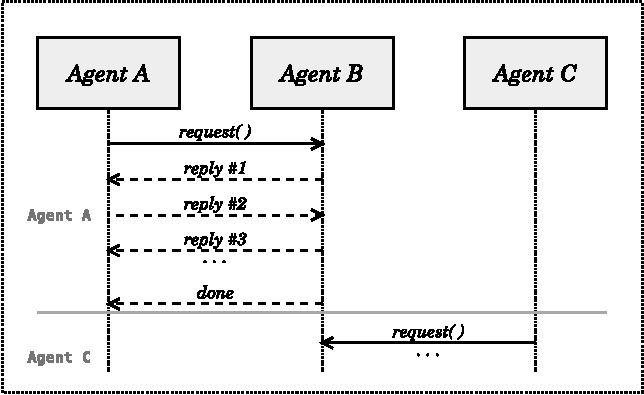
\includegraphics[width=\linewidth]{../figures/executionProblem.pdf}
			\caption{\small Acesso Direto}
			\label{fig:direct_method_execution}
	    \end{subfigure}
	    \begin{subfigure}[b]{.45\linewidth}
			\centering
			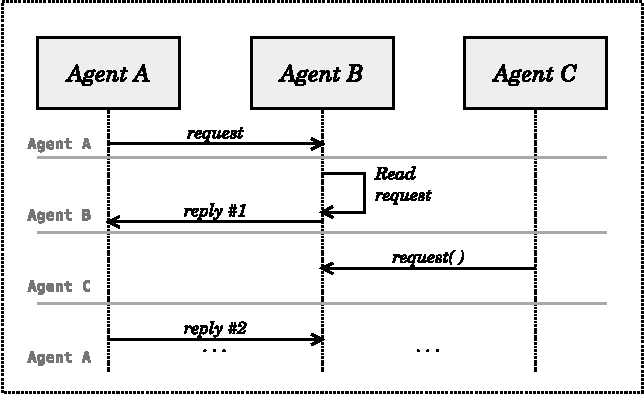
\includegraphics[width=\linewidth]{../figures/executionProblem2.pdf}
			\caption{\small Assíncrono}
			\label{fig:assynch_execution}
	    \end{subfigure}
	    \label{fig:execution_problems}
	\end{figure}

\end{frame}
\begin{frame}{SAJaS}
	Solução para communicação ``assíncrona'' no SAJaS
	\begin{figure}
		\centering
	    \begin{subfigure}[b]{0.45\linewidth}
			\centering
			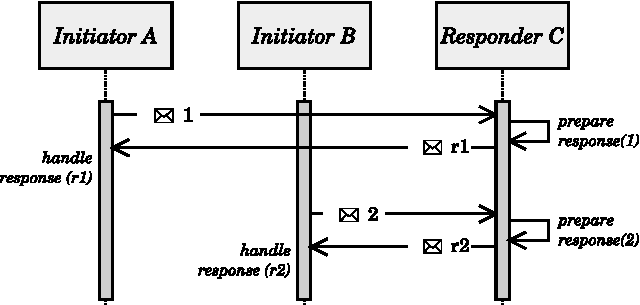
\includegraphics[width=\linewidth]{../figures/tickExample2.pdf}
			\caption{JADE}
			\label{fig:com-example-jade}
	    \end{subfigure}
	    \begin{subfigure}[b]{0.45\linewidth}
			\centering
			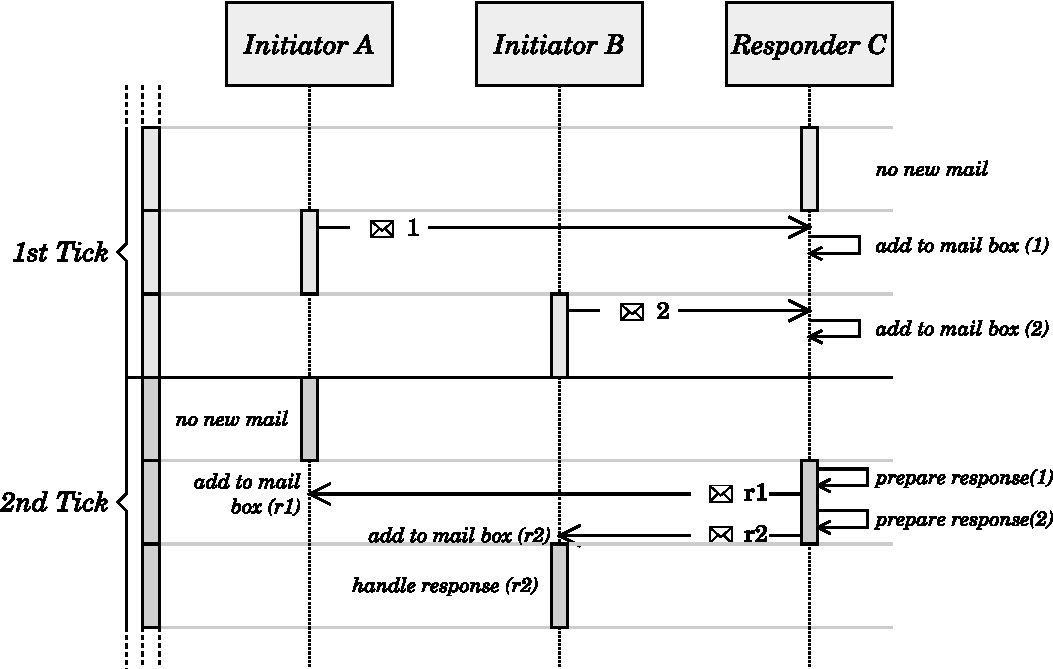
\includegraphics[width=\linewidth]{../figures/tickExample.pdf}
			\caption{SAJaS}
			\label{fig:com-example-repast}
	    \end{subfigure}
	    \caption{Communication and agent interaction}
	    \label{fig:execution_example}
	\end{figure}

\end{frame}

\subsection{Arquitetura}
\begin{frame}{Arquitetura}

\end{frame}

\subsection{FIPA}
\begin{frame}{FIPA}

\end{frame}

\section{MASSim2Dev}
%!TEX root = ../thesis.tex

%%%%%%%%%%%%%%%%%%%%%%%%%%%%%%%%%%%%%%%%%%%%%%%%%%%%%%
%%%%%%%%%%%%%%%%%%%%%%%%%%%%%%%%%%%%%%%%%%%%%%%%%%%%%%
\subsection{MASSim2Dev}
\begin{frame}{MASSim2Dev - Ferramenta de Conversão}

	\begin{itemize}
	\item MASSim2Dev (\emph{MAS Simulation to Development code conversion tool})
	\item Estabelece a ponte entre o desenvolvimento e simulação de MAS utilizando o SAJaS
	\end{itemize}
\end{frame}

\subsection{Transformações de código}
\begin{frame}{MASSim2Dev - Ferramenta de Conversão}

	Transformações de código Java: ferramentas estudadas

	\begin{itemize}
	\item ATL (``ATLAS Transformation Language'') - transformações de modelos através de AST usando linguagem específica;
	\item Spoon - transformações de código Java baseadas em anotações, usando Java
	\item \color{FEUPCor} JDT (``Eclipse Java Development Tools'') - criação de plugins para Eclipse, que permitem edições de alto nível, assim como via AST

	\end{itemize}
\end{frame}

\subsection{Processo de conversão}
\begin{frame}{MASSim2Dev - Ferramenta de Conversão}

	Após a conversão, não restam dependências da plataforma original.
	\begin{figure}[h]
		\centering
		\includegraphics[height=5cm]{../figures/conversion_representation.pdf}
	\end{figure}
\end{frame}

\begin{frame}{MASSim2Dev - Ferramenta de Conversão}

	Algoritmo
	\begin{samepage}
		\begin{enumerate}
		  \item Clonar o projeto selecionado
		  \item Mudar as referências a \emph{imports} em cada classe
		  \item Introduzir as bibliotecas necessárias (JADE, Repast...) e adiciona-las ao \emph{build path} do projeto
		  \item Reparar hierarquia (p.e. classes que estendem \texttt{RepastAgent} passam a estender \texttt{Agent})
		\end{enumerate}
	\end{samepage}
\end{frame}



\section{Validação}
%!TEX root = ../thesis.tex

%%%%%%%%%%%%%%%%%%%%%%%%%%%%%%%%%%%%%%%%%%%%%%%%%%%%%%
%%%%%%%%%%%%%%%%%%%%%%%%%%%%%%%%%%%%%%%%%%%%%%%%%%%%%%
\subsection{Validação}
\begin{frame}{Validação}
	Três testes de validação criados
	\begin{itemize}
		\item Rede contratual simples
		\item Rede contratual com multiplas sessões
		\item Jogo de tabuleiro RISK
	\end{itemize}

	Métricas avaliadas
	\begin{itemize}
		\item Resultado da execução do teste no SAJaS e no JADE
		\item Performance em ambos os casos
	\end{itemize}
\end{frame}

\subsection{}
\begin{frame}{Validação}
	Rede Contratual Simples

	\begin{figure}
		\centering
		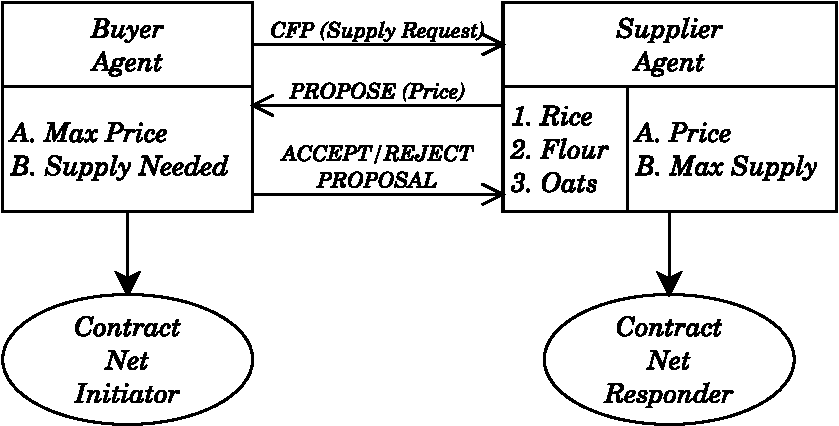
\includegraphics[height=2.3cm]{../figures/CNetExample.pdf}
	\end{figure}

	\begin{figure}
		\centering
		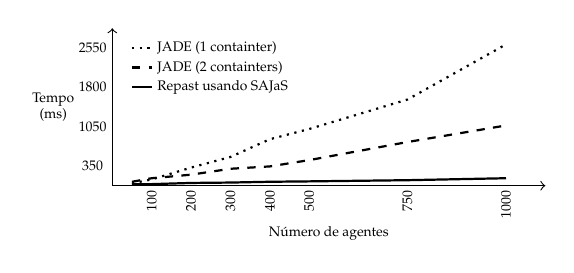
\begin{tikzpicture}[scale=0.50]
			\tiny
			% horizontal axis
			\draw[->] (0,0) -- (11,0);
			\draw (5.5,-1.2) node[align=center] {Número de agentes}; %label

			
			% labels
			\draw	%(0.5,0) node[rotate=90, anchor=east] {50}
					(1.0,0) node[rotate=90, anchor=east] {100}
					(2.0,0) node[rotate=90, anchor=east] {200}
					(3.0,0) node[rotate=90, anchor=east] {300}
					(4.0,0) node[rotate=90, anchor=east] {400}
					(5.0,0) node[rotate=90, anchor=east] {500}
					(7.5,0) node[rotate=90, anchor=east] {750}
					(10.,0) node[rotate=90, anchor=east] {1000};

			\draw	(-0.5,0.5) node[anchor=center] {350}
					(-0.5,1.5) node[anchor=center] {1050}
					(-0.5,2.5) node[anchor=center] {1800}
					(-0.5,3.5) node[anchor=center] {2550};
			% vertical axis
			\draw[->] (0,0) -- (0,4);
			\draw (-1.5,2) node[align=center] {Tempo\\(ms)}; %label
			%\draw (-1.5,1.6) node[align=center] {(ms)}; %label

			%% Data %%
			% JADE 2 containers
			\draw[thick,dashed] (0.5,3.0) --
				(1,3.0) node[anchor=west, pos=1.0] {JADE (2 containters)}; %subtitle
			\draw[thick,dashed] (0.5, 0.10) --
						(1.0, 0.19) --
						(2.0, 0.28) --
						(3.0, 0.43) --
						(4.0, 0.49) --
						(5.0, 0.65) --
						(7.5, 1.11) --
						(10., 1.53);
			% JADE 1 containers
			\draw[thick,dotted] (0.5,3.5) --
				(1,3.5) node[anchor=west, pos=1.0] {JADE (1 containter)}; %subtitle
			\draw[thick,dotted] (0.5, 0.06) --
						(1.0, 0.16) --
						(2.0, 0.46) --
						(3.0, 0.73) --
						(4.0, 1.18) --
						(5.0, 1.44) --
						(7.5, 2.19) --
						(10., 3.59);
			% Repast
			\draw[thick] (0.5,2.5) --
				(1,2.5) node[anchor=west, pos=1.0] {Repast usando SAJaS}; %subtitle
			\draw[thick] (0.5, 0.04) --
						(1.0, 0.04) --
						(2.0, 0.07) --
						(3.0, 0.08) --
						(4.0, 0.10) --
						(5.0, 0.11) --
						(7.5, 0.14) --
						(10., 0.19);
		\end{tikzpicture}
	\end{figure}
\end{frame}

\subsection{}
\begin{frame}{Validação}
	Rede contratual com múltiplas sessões. Gráficos: sucesso médio em 5 execuções ao longo 2000 contratos no SAJaS (cima) e no JADE (baixo)
	\vspace{-0.5cm}
	\begin{figure}
		\centering
		\begin{subfigure}[b]{\textwidth}
			\centering
			\begin{tikzpicture}[scale=0.4]
				\tiny

				% horizontal axis
				\draw[->] (0,0) -- (11,0);
				\draw (5.5,-1.2) node[align=center] {Número de Contratos}; %label

				% labels
				\draw	(0  ,0) node[anchor=north] {0}
						(2.5,0) node[anchor=north] {500}
						(5  ,0) node[anchor=north] {1000}
						(7.5,0) node[anchor=north] {1500}
						(10 ,0) node[anchor=north] {2000};
				
				
				% vertical axis
				\draw[->] (0,0) -- (0,5);
				\draw (-1.1,2.5) node[rotate=90, anchor=south, align=center]
					{\% de sucesso}; %label
				\draw	(0, 1) node[anchor=east] {0.25}
						(0, 2) node[anchor=east] {0.50}
						(0, 3) node[anchor=east] {0.75}
						(0, 4) node[anchor=east] {1.00};
				
				

				%% Data %%

				%subtitles
				\draw[thick] (0.5,3.5) --
					(1,3.5) node[anchor=west, pos=1.0] {Usando confiança};
				\draw[thick, dotted]
					(0.5,4.5) --
					(1,4.5) node[anchor=west, pos=1.0] {Usando apenas o preço}; 

				%lines
				\input{../chapters/charts/enterprise_values_jade}


			\end{tikzpicture}
		\end{subfigure}
		\vspace{0.1cm}\\
		\begin{subfigure}[b]{\textwidth}
			\centering
			\begin{tikzpicture}[scale=0.4]
				\tiny

				% horizontal axis
				\draw[->] (0,0) -- (11,0);
				\draw (5.5,-1.2) node[align=center] {Número de contratos}; %label

				% labels
				\draw	(0  ,0) node[anchor=north] {0}
						(2.5,0) node[anchor=north] {500}
						(5  ,0) node[anchor=north] {1000}
						(7.5,0) node[anchor=north] {1500}
						(10 ,0) node[anchor=north] {2000};
				
				
				% vertical axis
				\draw[->] (0,0) -- (0,5);
				\draw (-1.1,2.5) node[rotate=90, anchor=south, align=center]
					{\% de sucesso}; %label
				\draw	(0, 1) node[anchor=east] {0.25}
						(0, 2) node[anchor=east] {0.50}
						(0, 3) node[anchor=east] {0.75}
						(0, 4) node[anchor=east] {1.00};

				%% Data %%

				%subtitles
				\draw[thick] (0.5,3.5) --
					(1,3.5) node[anchor=west, pos=1.0] {Usando trust};
				\draw[thick, dotted] 
					(0.5,4.5) --
					(1,4.5) node[anchor=west, pos=1.0] {Usando apenas o preço}; 
				
				%lines
				\input{../chapters/charts/enterprise_values_sajas}


			\end{tikzpicture}
		\end{subfigure}
	\end{figure}
\end{frame}

\subsection{}
\begin{frame}{Validação}
	Jogo de tabuleiro RISK. Gráfico: performance de um jogo de Risk com 5 agentes durante 8 segundos.
	\begin{figure}
		\begin{subfigure}[b]{0.5\textwidth}
			\begin{tikzpicture}[scale=0.40]
			\tiny
				% horizontal axis
				\draw[->] (0,0) -- (11,0);
				\draw (5.5,-1.2) node[align=center] {Tempo/s}; %label

				% labels
				\draw	(1.25,0) node[anchor=north] {1}
						(2.5,0)	 node[anchor=north] {2}
						(3.75,0) node[anchor=north] {3}
						(5,0)	 node[anchor=north] {4}
						(6.25,0) node[anchor=north] {5}
						(7.5,0)	 node[anchor=north] {6}
						(8.75,0) node[anchor=north] {7}
						(10,0)	 node[anchor=north] {8};
				
				% vertical axis
				\draw[->] (0,0) -- (0,5);
				\draw (-1.1,2.5) node[rotate=90, anchor=south, align=center]
					{Número de rondas}; %label
				\draw	(0, 1) node[anchor=east] {30}
						(0, 2) node[anchor=east] {60}
						(0, 3) node[anchor=east] {90}
						(0, 4) node[anchor=east] {120};

				%% Data %%

				%subtitle
				\draw[thick,thick] (0.5,3.5) --
					(1,3.5) node[anchor=west, pos=1.0] {SAJaS};
				%line
				\draw[thick, dotted]%subtitle
					(0.5,4.5) --
					(1,4.5) node[anchor=west, pos=1.0] {JADE}; 
				\input{../chapters/charts/risk_times}

			\end{tikzpicture}
		\end{subfigure}
		\begin{subfigure}[b]{0.5\textwidth}
			\centering
			\includegraphics[height=3cm]{../figures/risk_GUI.png}
		\end{subfigure}
	\end{figure}
\end{frame}


\section{Conclusões}
%!TEX root = ../thesis.tex
\chapter{Conclusions}
\label{chap:conclusions}

MAS are used in many different domains and research based on simulation has seen an increase in the use of agent-based approaches in their development. As a result, many frameworks for the development of MABS have been created. With a review of the available literature, it is possible to conclude that there is interest in bridging the domains of MAS and MABS. While MABS are typically not used in production, MAS are usually not the most appropriate to perform tests and simulations, more so when large number of agents are in use.

Some works were studied whose motivation was to bridge these domains. MISIA, JRep and PlaSMA proposed approaches that extended the MAS development framework JADE with simulation development features. This thesis proposed an alternative approach in which JADE-based features were included in the MAS framework Repast without relying in JADE libraries -- those features were re-implemented for this purpose.

\section{Main Contributions}
To bridge the gap between MAS development and simulation, the Simple API for JADE-based Simulations (\apiname) was created. JADE developers are able to create Repast-based simulations using familiar JADE features. The \pluginname (\plugin) was also developed to enable the conversion of simulations created with \apiname into JADE MAS.

The main issues detected during the development of \apiname were related to to the different nature of the execution of Repast and JADE. JADE's agents run in multiple threads and global agent synchronization does not exist. Agent interaction happens asynchronously. The kind of simulation frameworks targeted by this API, like Repast, relies on synchronized events that occur consecutively in ``ticks''. By using ACLMessages in Repast and a messaging system that relies on messages being kept in a mail queue, asynchronous agent interaction is possible despite Repast synchronism. Messages are processed when the simulation grants execution the the agent who owns them.

Negotiation scenarios were created to validate both \apiname and \plugin. The goals were to demonstrate that it was possible to create agent-based scenarios with some complexity using \apiname's implemented features and that after its conversion using \plugin was not only feasible, but the resulted MAS displayed identical behaviour when executed. Furthermore, the \apiname version is significantly faster. The two negotiation scenarios showed that a Repast simulation based on \apiname was many times faster than its JADE equivalent.

%!TEX root = ../thesis.tex
\chapter{Future Work}
\label{chap:futurework}



\section{Referências}
\begin{frame}{Referências}
\bibliographystyle{apacite}
\bibliography{myrefs}
\end{frame}


\end{document}

